% Draft of the tests results

With the predefined poses in Table \ref{table-groupA} and Table \ref{table-groupB}, we obtained the computed joint wrench from offline PC (JointWrench\_PC) and computed joint wrench from reading robot base in real time (JointWrech\_Base). The $i^{th}$ joint wrench contains force and torque along x, y and z axis of $i^{th}$ joint frame. The difference of these two joint wrench values is defined as: $JointWrench\_Error = JointWrench\_PC - JointWrech\_Base$

\begin{figure}
	\begin{center}
		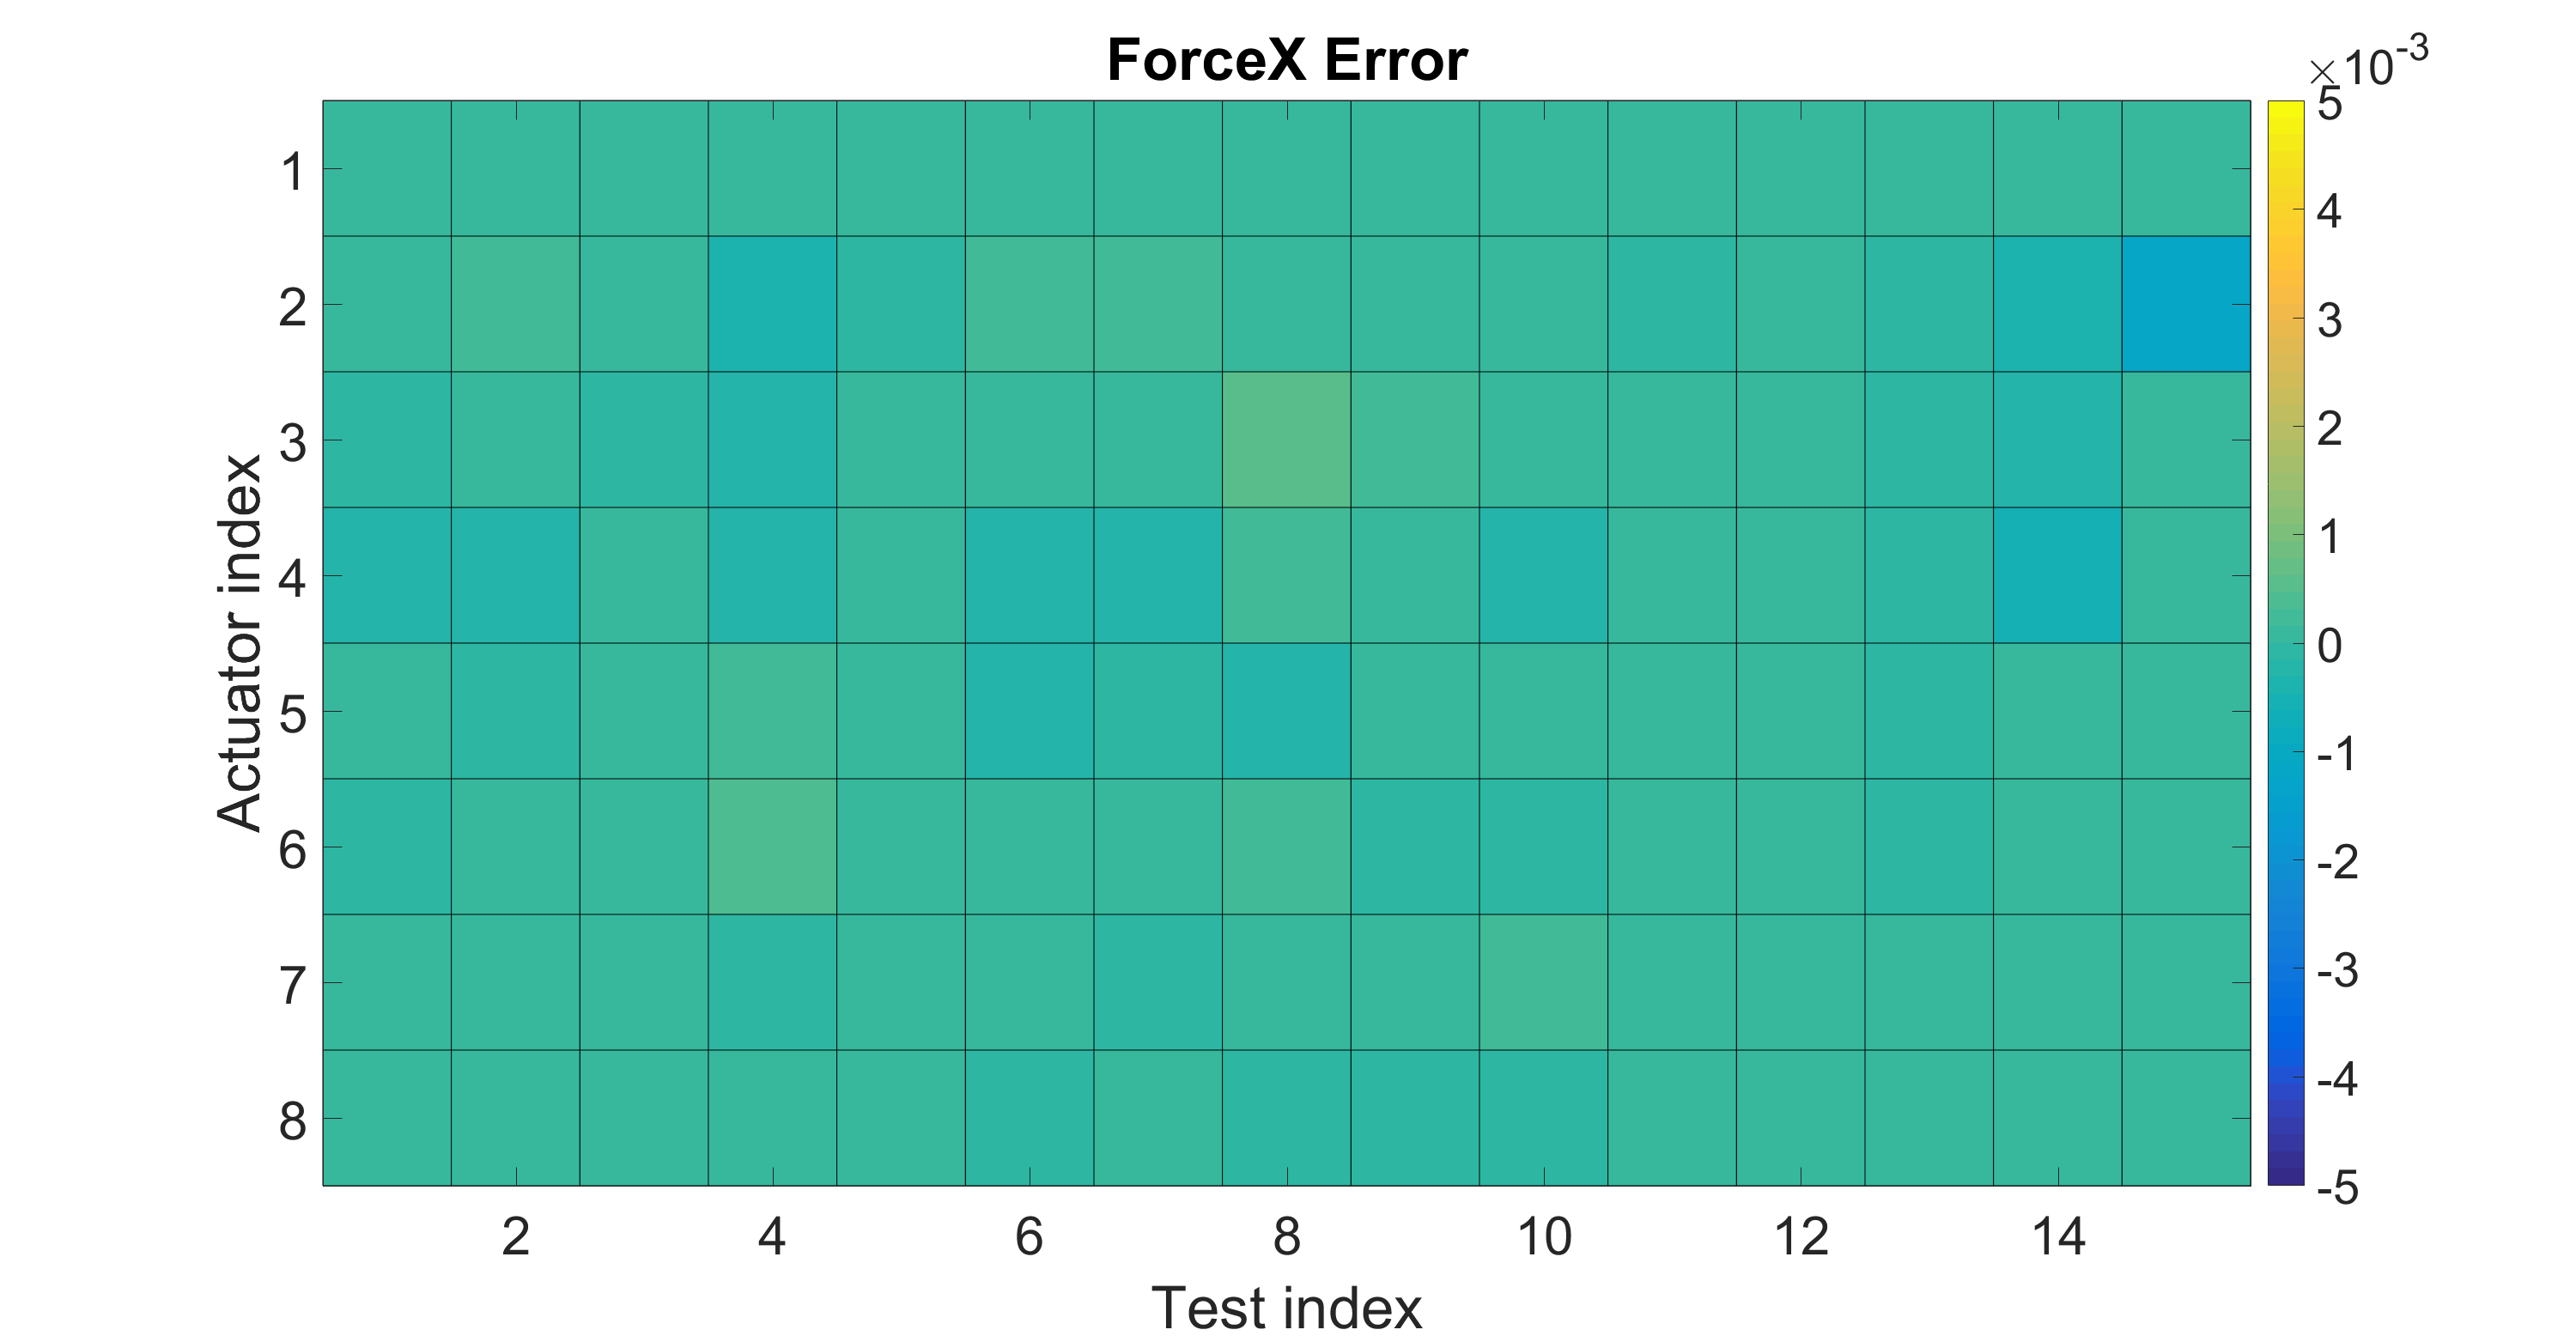
\includegraphics[width=0.9\textwidth]{./images/Result1.png}%
		\caption{Difference of Force along X axis}
		\label{fig:forcex}%
	\end{center}
\end{figure}

\begin{figure}
	\begin{center}
		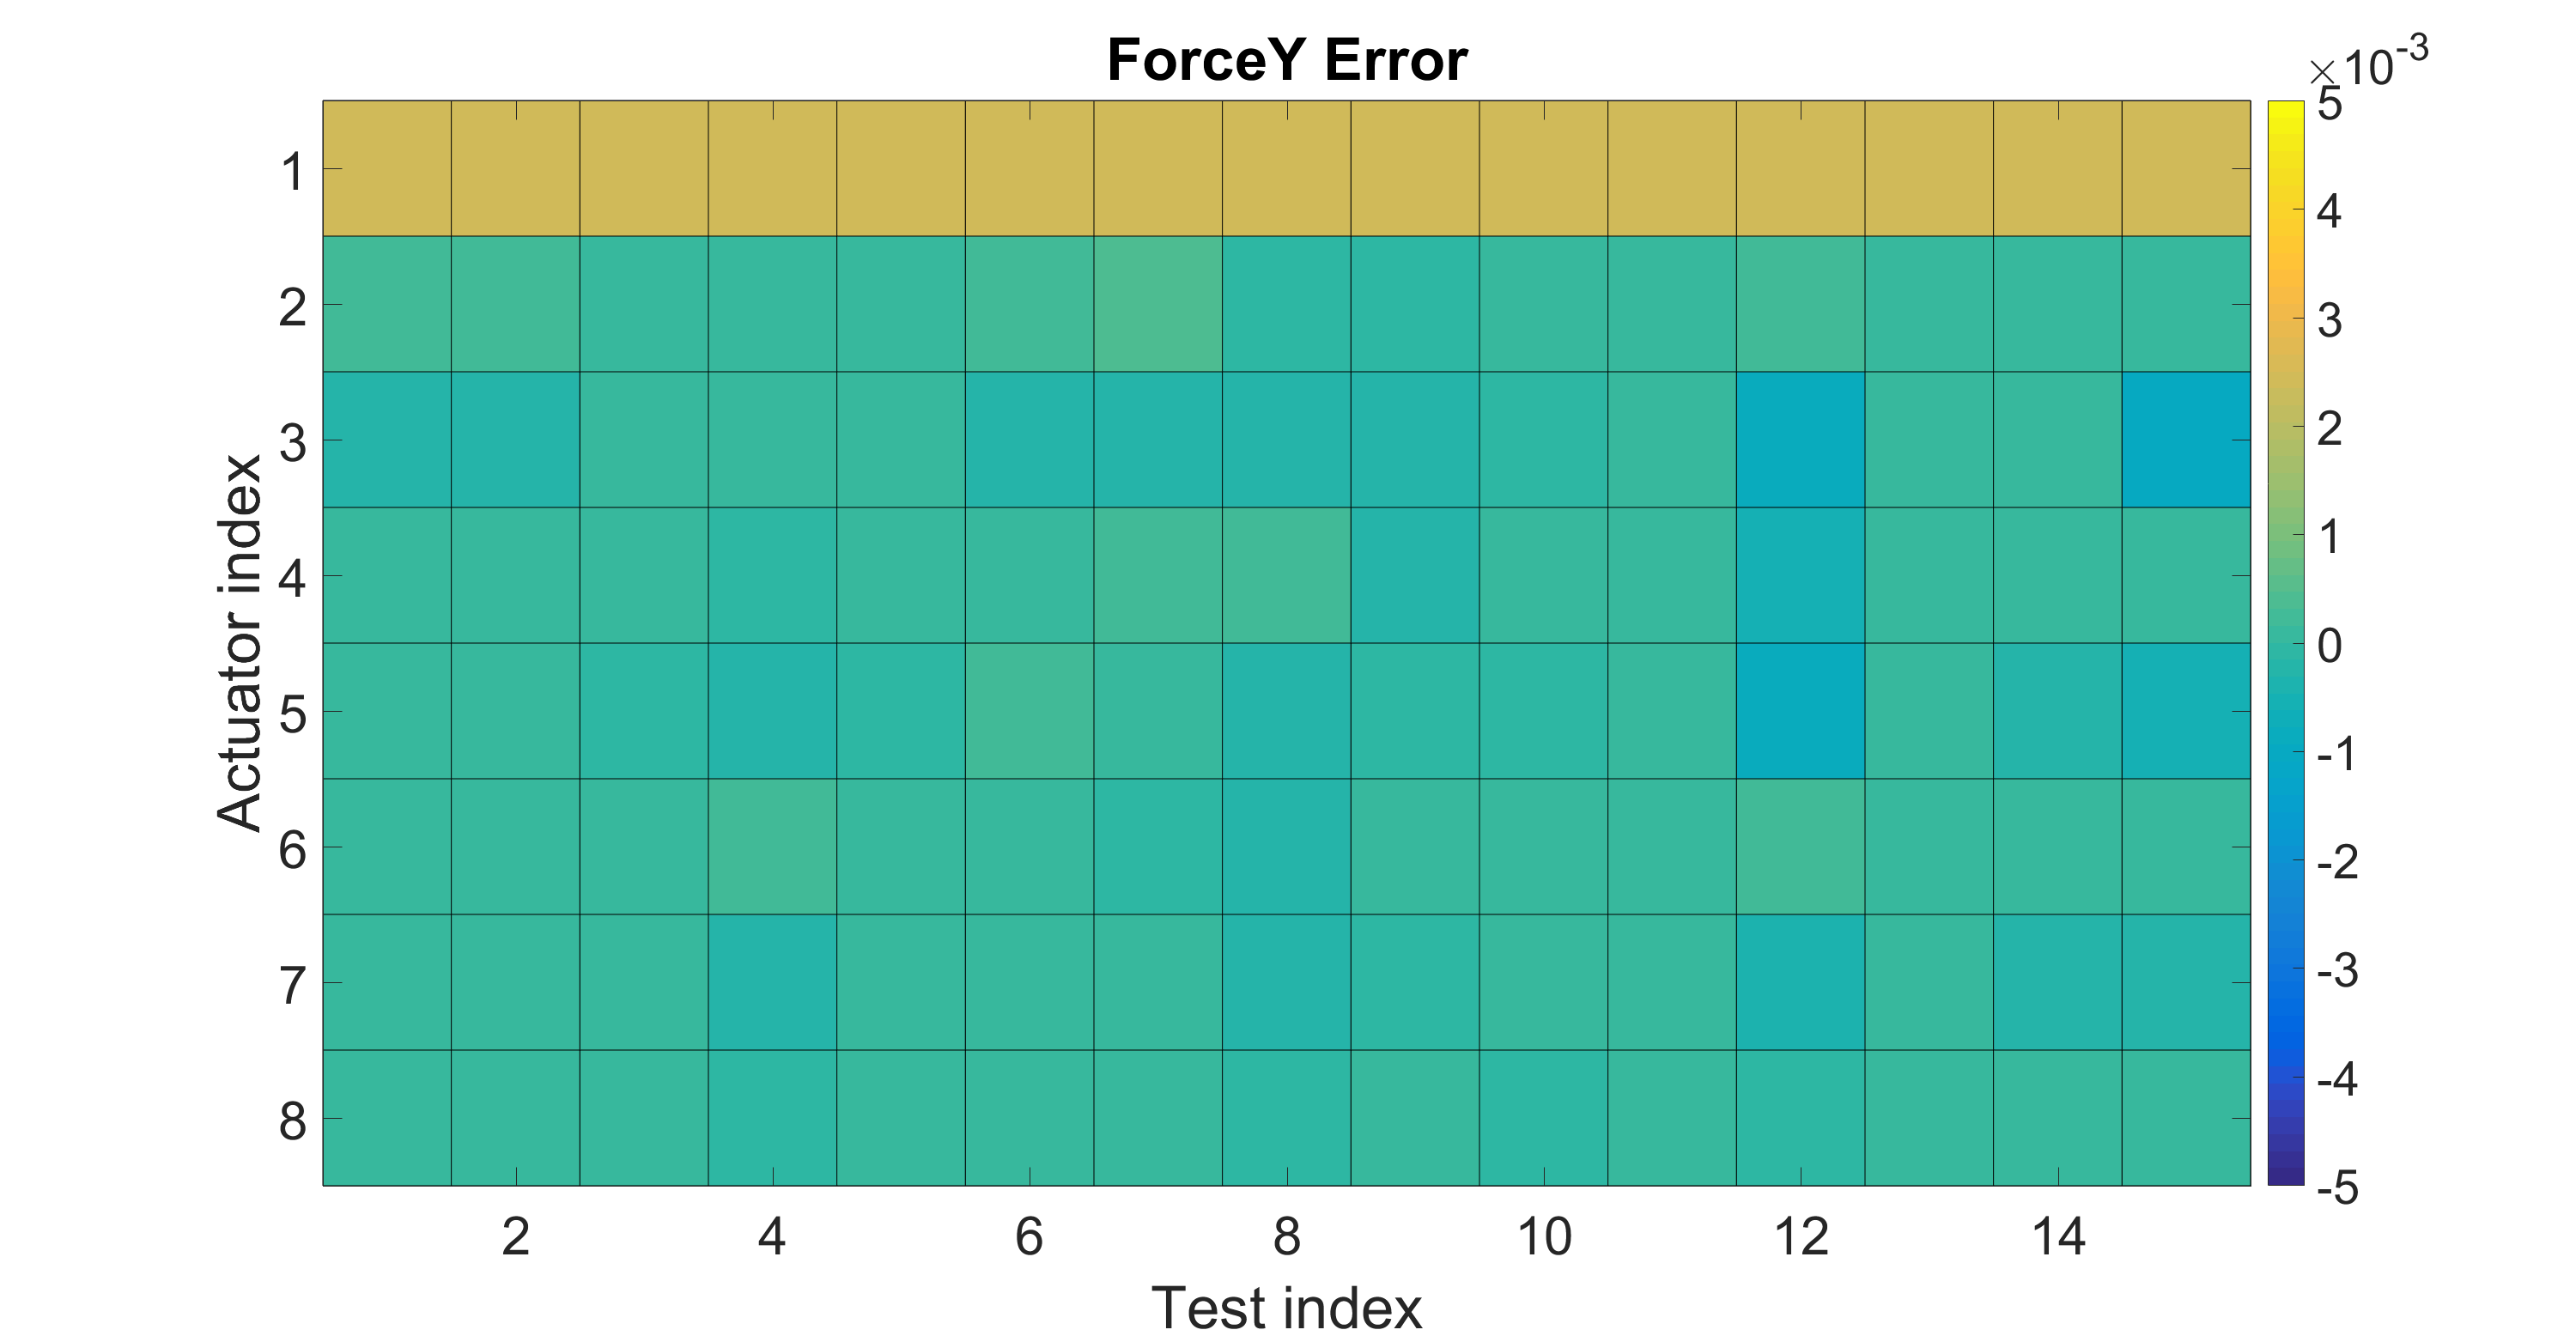
\includegraphics[width=0.9\textwidth]{./images/Result2.png}%
		\caption{Difference of Force along Y axis}
		\label{fig:forcey}%
	\end{center}
\end{figure}

\begin{figure}
	\begin{center}
		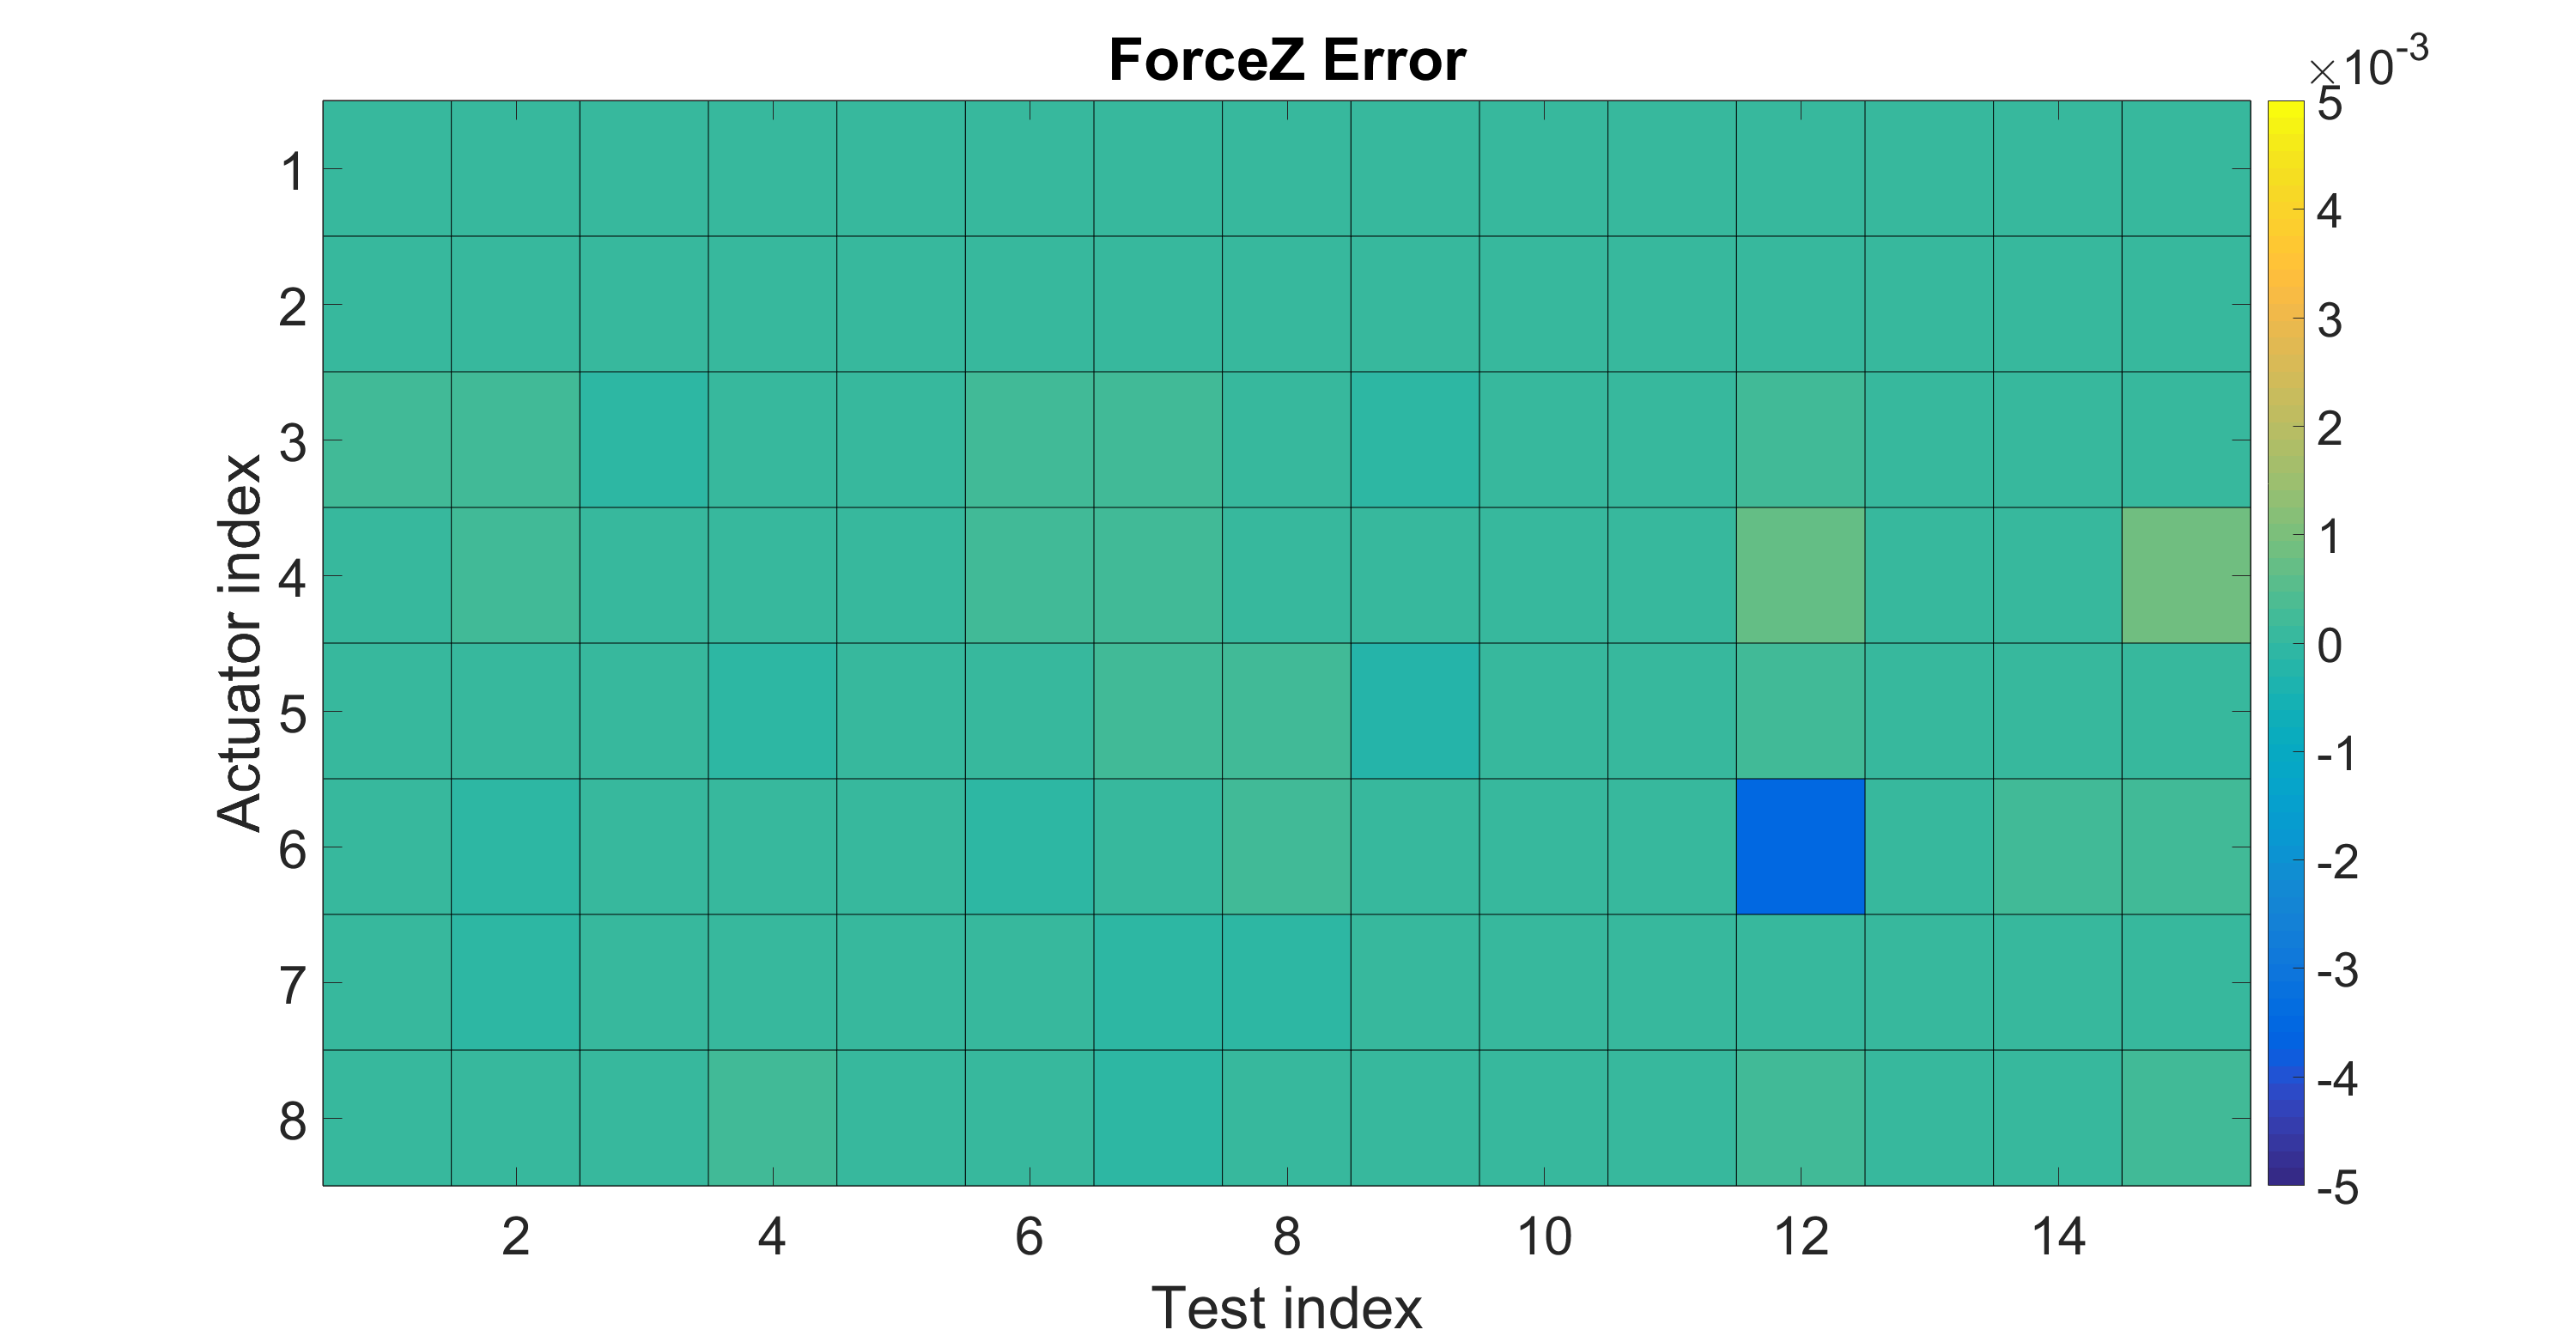
\includegraphics[width=0.9\textwidth]{./images/Result3.png}%
		\caption{Difference of Force along Z axis}
		\label{fig:forcez}%
	\end{center}
\end{figure}

\begin{figure}
	\begin{center}
		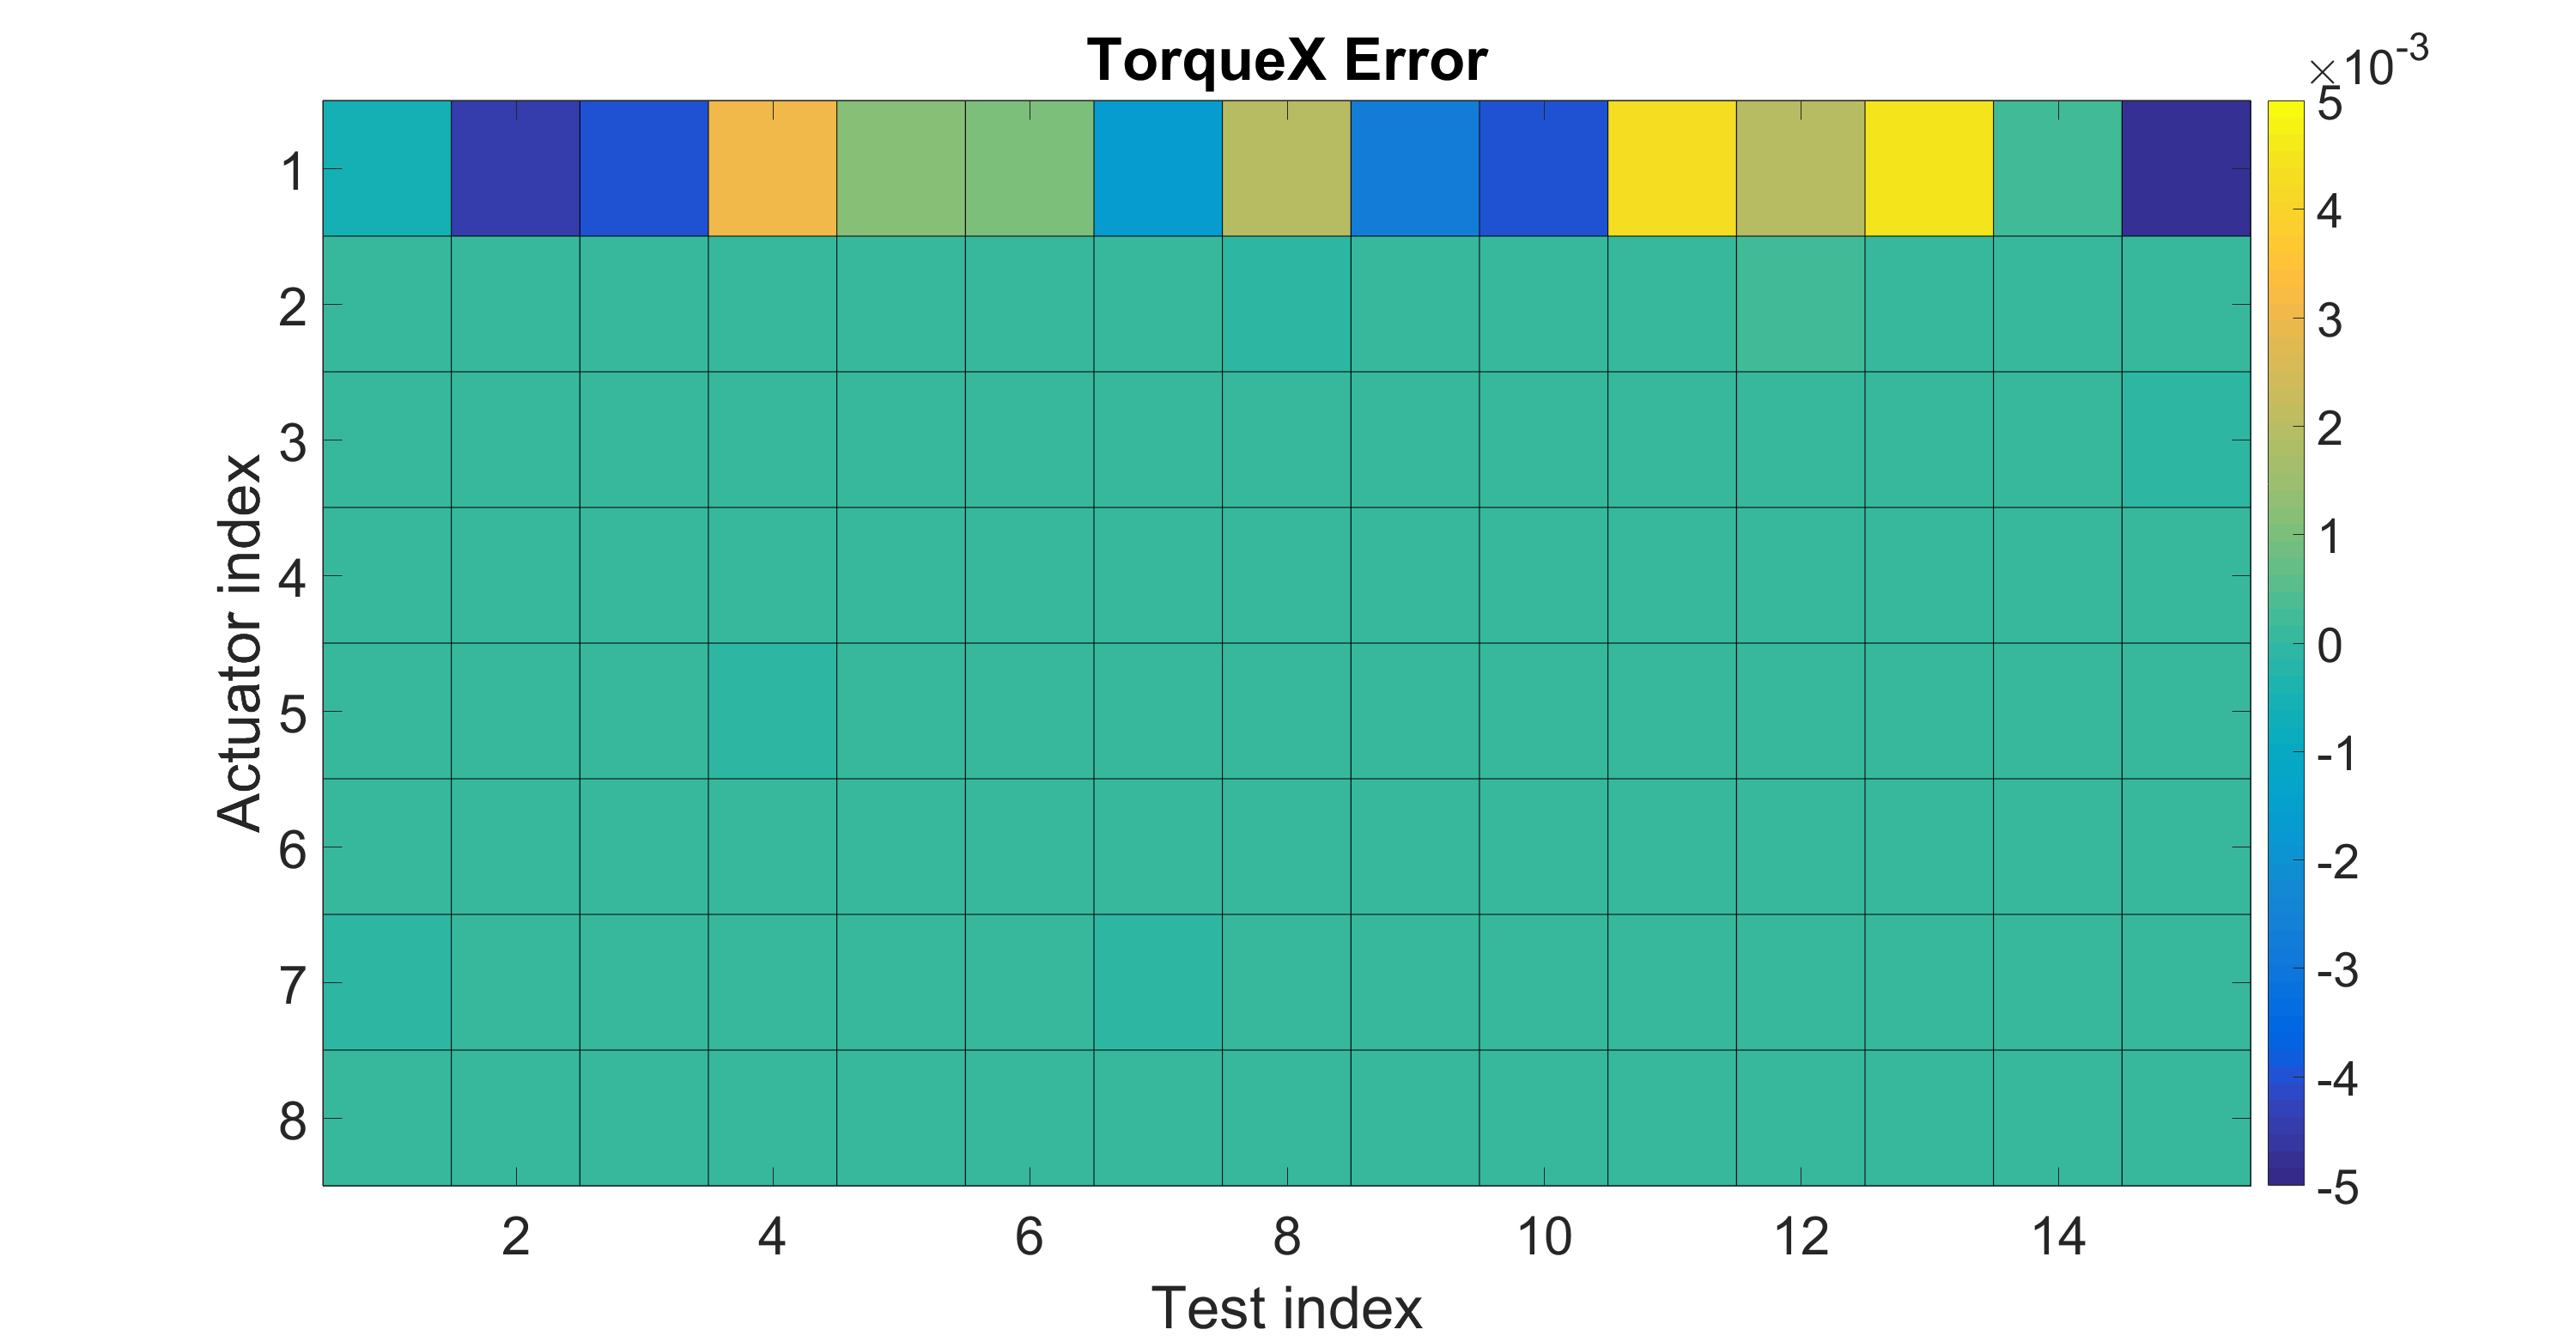
\includegraphics[width=0.9\textwidth]{./images/Result4.png}%
		\caption{Difference of Torque along X axis}
		\label{fig:torquex}%
	\end{center}
\end{figure}

\begin{figure}
	\begin{center}
		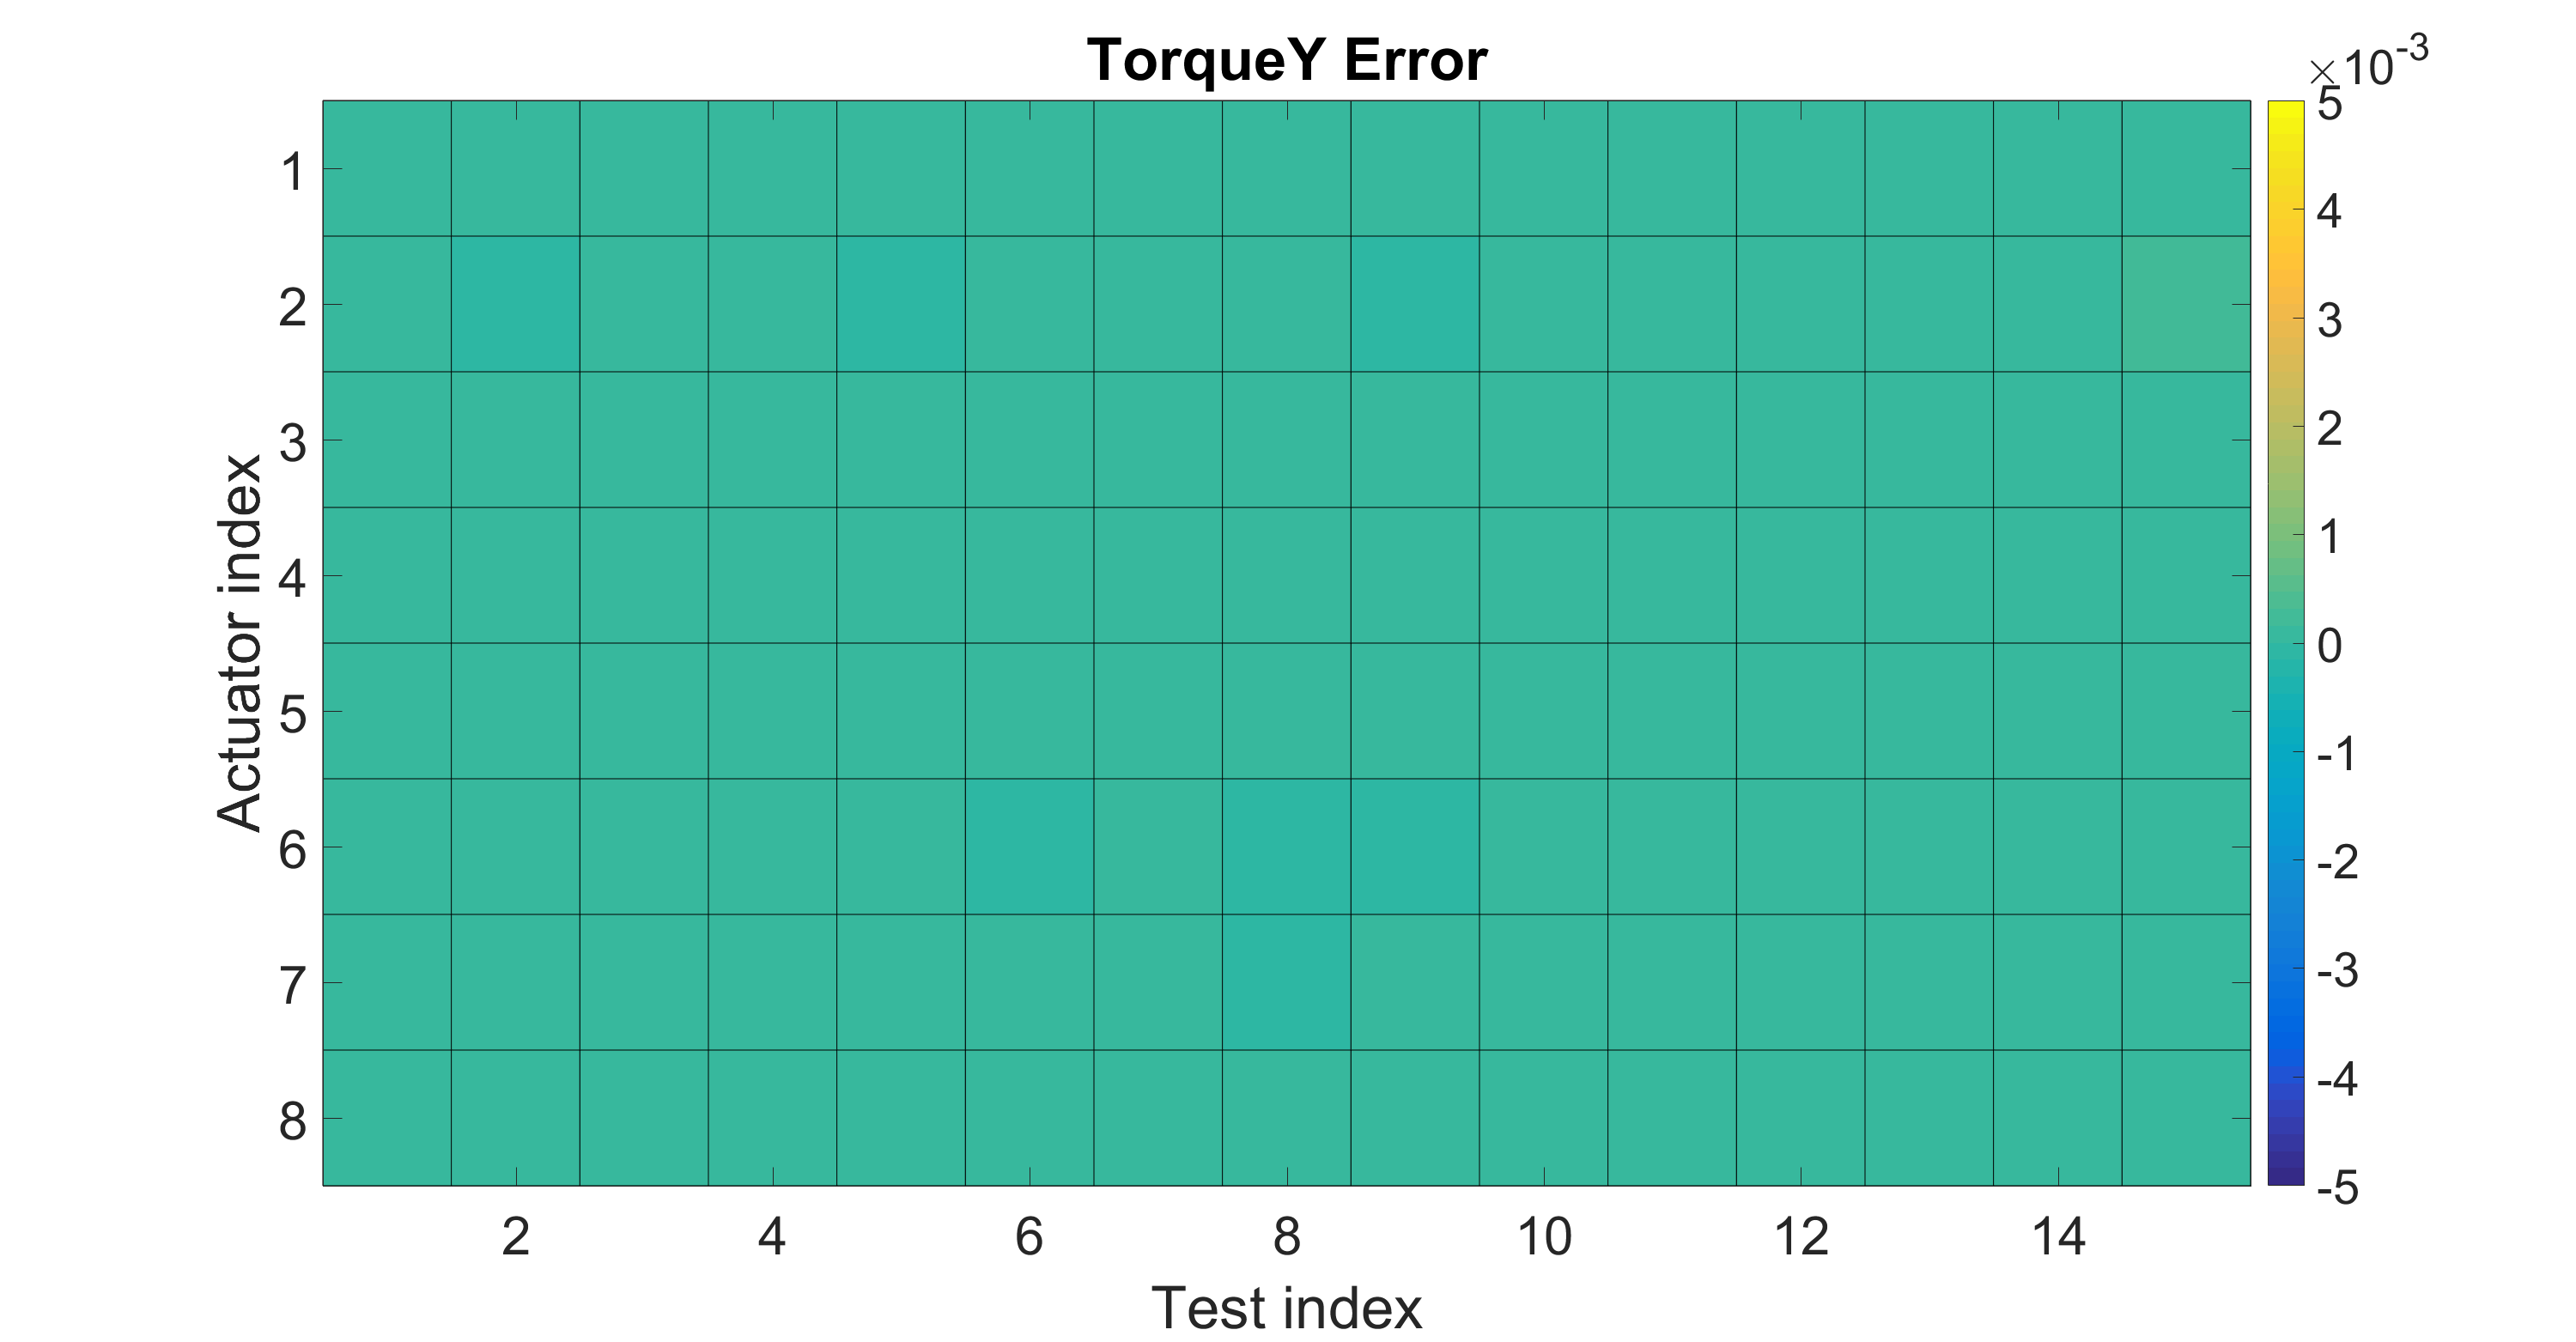
\includegraphics[width=0.9\textwidth]{./images/Result5.png}%
		\caption{Difference of Torque along Y axis}
		\label{fig:torquey}%
	\end{center}
\end{figure}

\begin{figure}
	\begin{center}
		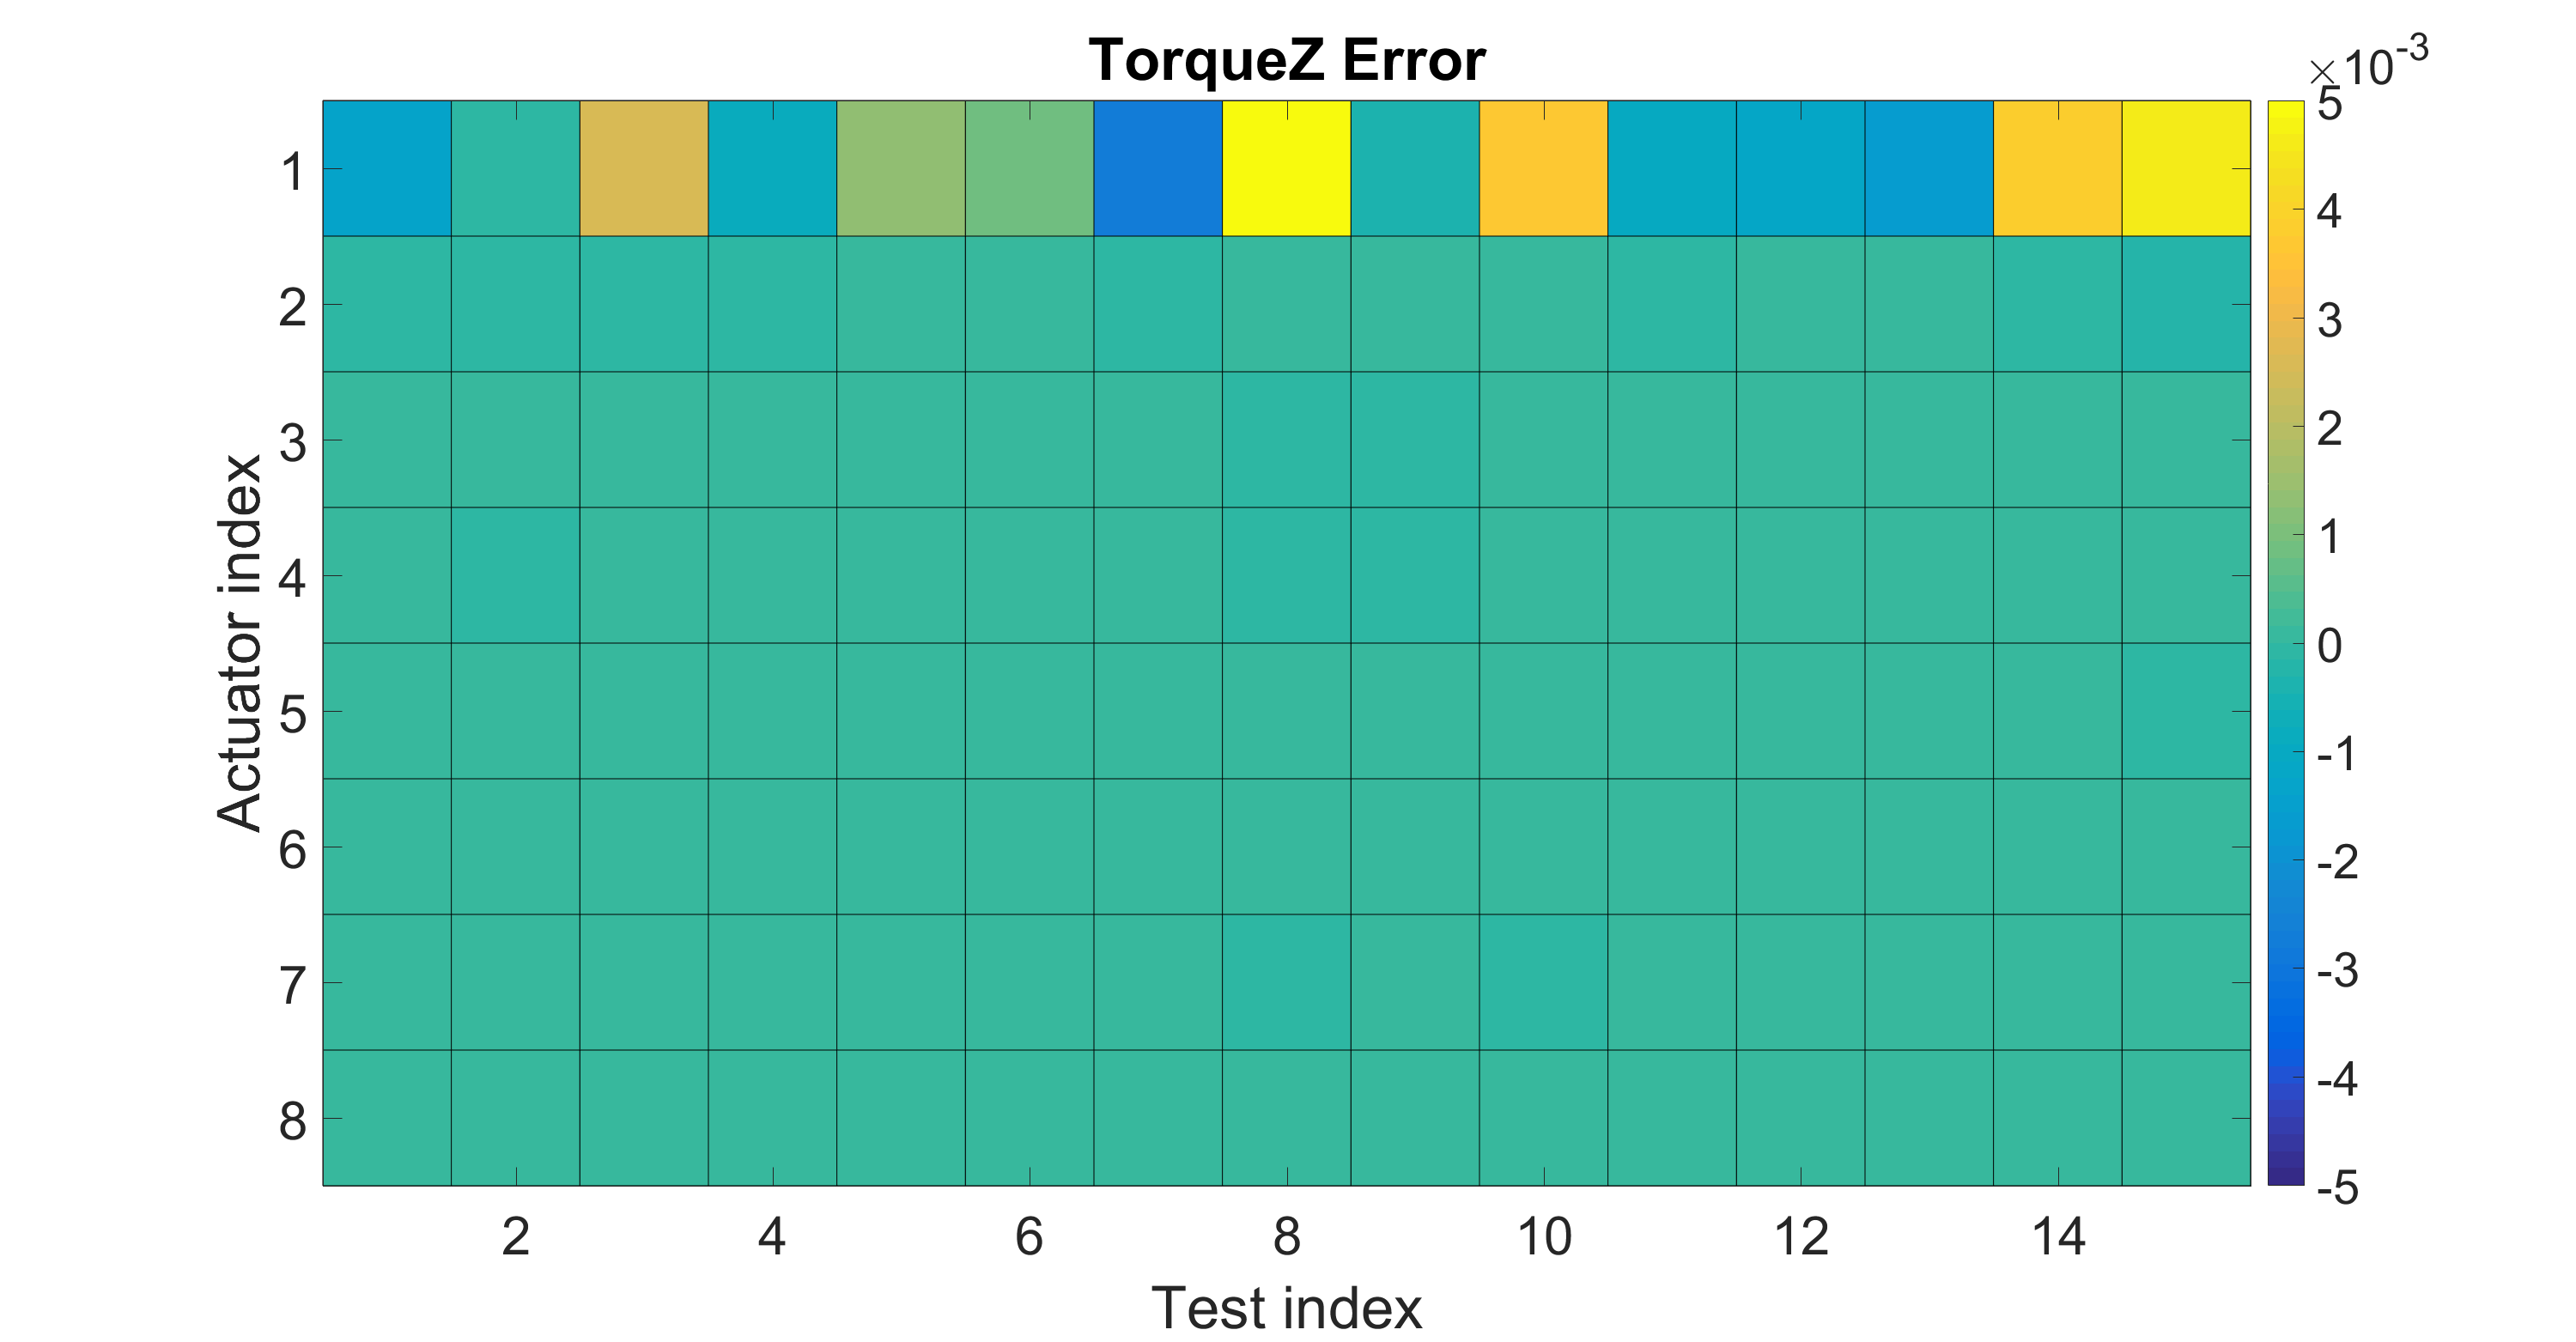
\includegraphics[width=0.9\textwidth]{./images/Result6.png}%
		\caption{Difference of Torque along Z axis}
		\label{fig:torquez}%
	\end{center}
\end{figure}

The Figure \ref{fig:forcex} to Figure \ref{fig:torquez} shows the error distribution of all the tests in 15 poses (horizontal axis). The vertical axis indicates the joint index, with base with index 1 and joint 7 with index 8. The color of each cell demonstrates the error of the corresponding test according to the colorbar on the right. It is obvious that JointWrench\_Error is very small, in the scale of $10^{-3}$ N (Force) or Nm(Torque). In other words, the JointWrench\_PC and JointWrech\_Base have very close values. The sightly differences may due to the residue between robot position command and feedback, as well as numerical errors in the computation. Notable errors happened to the robot base (index 1 of the vertical axis). The cause is NOVA provide 2 decimal values for the wrench at the base, while 4 decimal values at other joints. The omitted decimal values cause error in the scale of $10^{-3}$. 

In conclusion, the joint wrench data from robot base matches with the data from offline PC. The computed joint wrench in robot base performs as designed.